\documentclass{beamer}
\usepackage[english,russian]{babel}
\usepackage[utf8]{inputenc}
\usepackage{pagenumber}

\usepackage{hyperref}
% Стиль презентации
\usetheme[numbers, totalnumbers]{Dresden}
% цветовая схема
\usecolortheme{beaver}

\makeatletter
\defbeamertemplate*{footline}{Dresden}{
	\leavevmode%
	\hbox{%
	\begin{beamercolorbox}[wd=.3\paperwidth,ht=3.00ex,dp=1ex,center]{author in head/foot}%
		\usebeamerfont{author in head/foot}%
		\insertauthor	
	\end{beamercolorbox}%
	\begin{beamercolorbox}[wd=0.5\paperwidth,ht=3.00ex,dp=1ex,center]{title in head/foot}%
		\usebeamerfont{title in head/foot}\inserttitle
	\end{beamercolorbox}%
	\begin{beamercolorbox}[wd=.2\paperwidth,ht=3.00ex,dp=1ex,right]{date in head/foot}%
		\usebeamerfont{date in head/foot}\hspace*{2em}
		\insertframenumber{} / \inserttotalframenumber\hspace*{2ex}
	\end{beamercolorbox}}%
}
\makeatother

\begin{document}
\title{Оптимизация проверки задач для Linux* курсов}  
\author{Волков Д., Заславский М.}
\institute{Computer Science Center}
\date{\today} 
% Создание заглавной страницы
\frame{\titlepage} 

\begin{frame}{Stepic}
	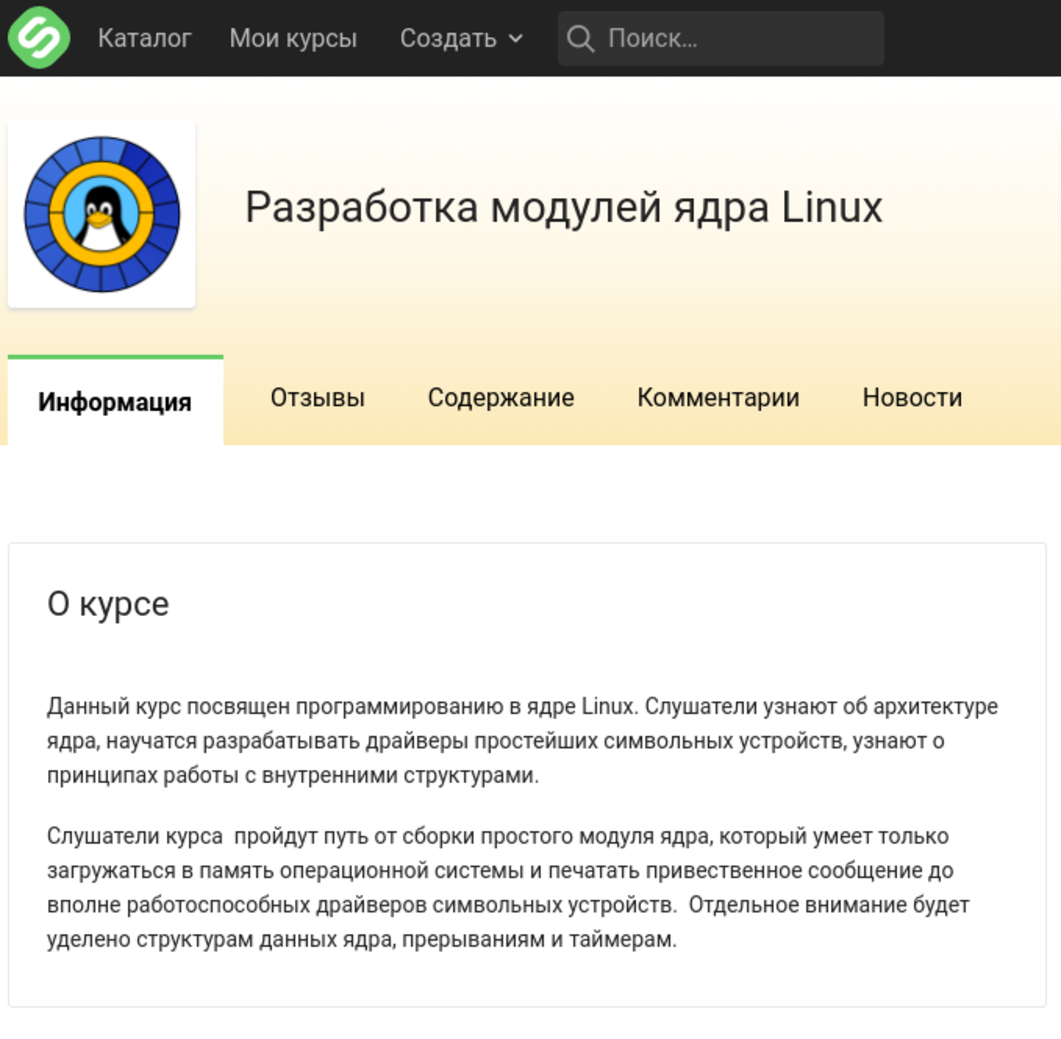
\includegraphics[width=100mm]{./stepic.pdf}
\end{frame}

\begin{frame}{Зачем?}
	\begin{itemize}
		\item Облегчить задачу составителям курсов
		\item Отделение проверяющей системы от тестов
		\item Сокращение времени ожидания вердикта пользователем
	\end{itemize}
\end{frame}

\begin{frame}{Цели и задачи}
	\textbf{Цель проекта:} оптимизация структуры и производительности проверяющей системы.

	\textbf{Задачи:}
	\begin{itemize}
		\item Архитектурное разделение проверяющей системы и сценариев проверки отдельных заданий.
		\item Профилирование проверки решений
		\item Ускорение проверки решений 
	\end{itemize}
\end{frame}

\begin{frame}{На старте}
	Проблема, связанная с взаимосвязью проверяющей системы
	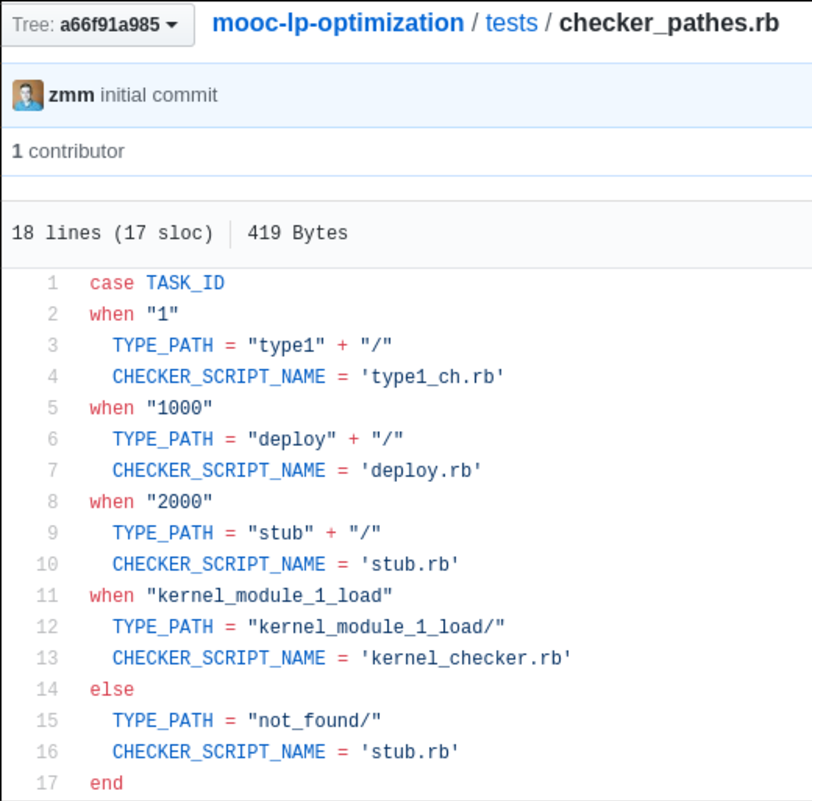
\includegraphics[width=80mm]{./patchesrb.pdf}
\end{frame}

\begin{frame}{На старте}
	Виртуализация \textbf{KVM + Libvirt}
	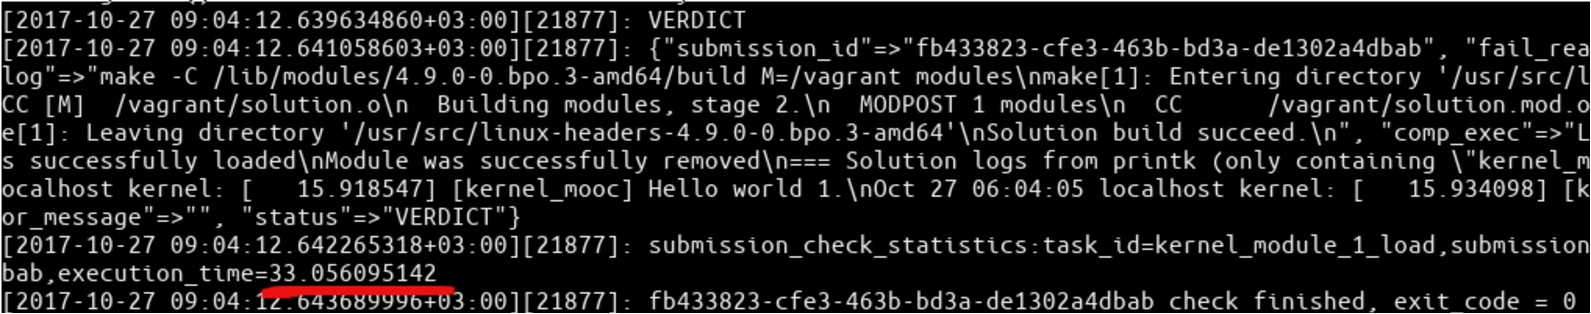
\includegraphics[width=115mm]{./length_start.pdf}
\end{frame}

\begin{frame}{Оптимизация архитектуры}
	\begin{itemize}
		\item Рефакторинг кодовой базы
		\item Отделение чекеров от проверяющей системы
	\end{itemize}
\end{frame}

\begin{frame}{Профилирование}
	Парсинг логов \textit{pdaemon.sh}
	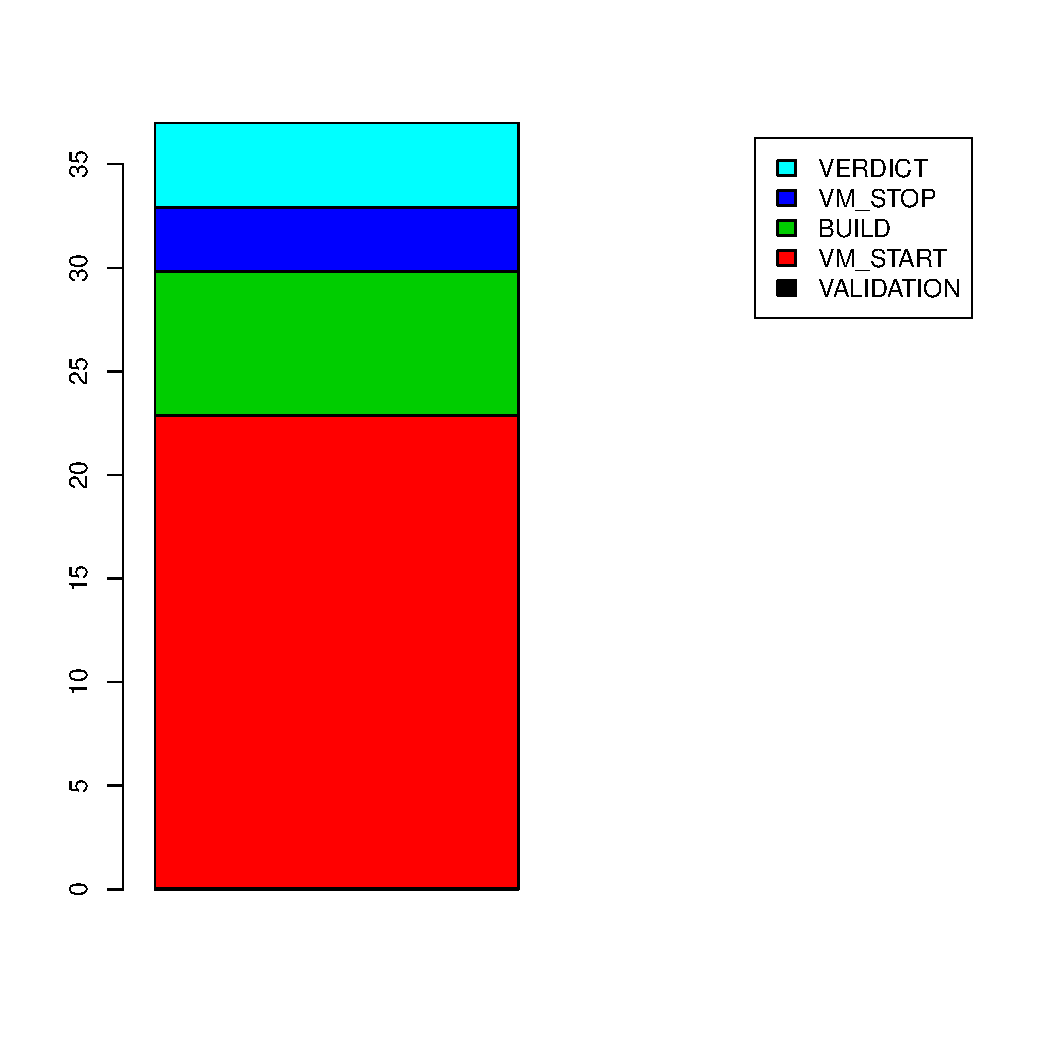
\includegraphics[width=70mm]{./libvirt_bar.pdf}
\end{frame}

\begin{frame}{Профилирование}
	Парсинг логов \textit{pdaemon.sh}
	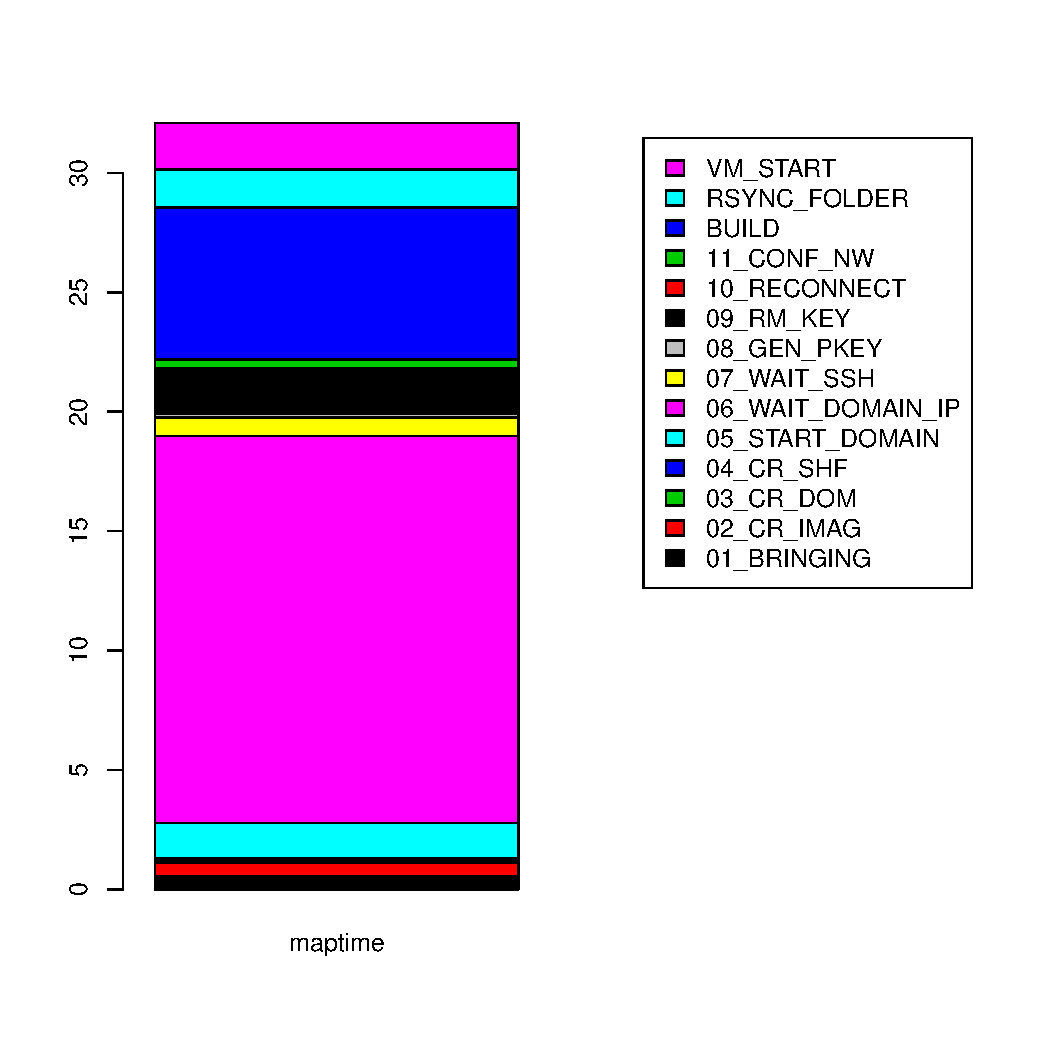
\includegraphics[width=70mm]{./vm_start_bar.pdf}
\end{frame}

\begin{frame}{Оптимизация по времени}
	\textit{will be done}
\end{frame}

\begin{frame}{Технологии}
	\begin{itemize}
		\item ОС (гостевая и хостовая): \textbf{GNU/Linux}
		\item Виртуализация: \textbf{QEMU/KVM}, \textbf{Vagrant} + (\textbf{Docker} || \textbf{Libvirt})
		\item Языки: \textbf{Ruby}, \textbf{Python}, \textbf{Bash}, \textbf{R}
		\item Система контроля версий: \textbf{Git}
		\item Удаленный доступ: \textbf{SSH}
		\item Коммуникация: \textbf{Slack}
	\end{itemize}
\end{frame}

\begin{frame}{Результаты}
	\begin{itemize}
		\item Проверяющая система отделена от тестовых сценариев
		\item Создание автоматических тестов производительности системы
		\item Ускорение проверки!
	\end{itemize}
\end{frame}

\begin{frame}{Перспективы}
	Проект не завершен в полной мере, ещё есть направления для развития:
	\begin{itemize}
		\item Интеграция изменений
		\item Автоматические тесты производительности могут быть совершеннее
		\item Дальнейший рефакторинг кода
		\item Потенциально возможно дальнейшее ускорение проверки
	\end{itemize}
\end{frame}

\begin{frame}{Ссылки}
	На курсы на степике, возможно ссылку на репозиторий с патчами
	\begin{itemize}
		\item \textbf{https://github.com/OSLL/mooc-lp-optimization}
	\end{itemize}
\end{frame}

\end{document}
